
\chapter{Movement}
\label{cha:movement}

In Chap.~\ref{chTutorial} we showed how to move your agent through the
{\tt Cerebellum}, which you need to provide joint velocities. \libbats
provides an interface to create special modules to determine these
velocities and create coordinated movements, in the form of the {\tt
  JointController} class, with a few specific implementations. We will
discuss these here.

\section{{\tt JointController}}
\label{sec:tt-jointcontroller}

The {\tt JointController} class is a very basic interface that
provides two-step semantics for generating angular velocities for
joints: first, the controller is run by calling the virtual {\tt
  run()} method, which should fill the {\tt d\_jointVelocities}
vector. Secondly, this vector is requested through the {\tt
  getJointVelocities()} method, which can then be used to build
actions and feed these to the Cerebellum, as discussed before. So,
specific implementations must implement the {\tt run()} method, which
then should be called at every think cycle. The {\tt run()} method
takes a pointer to an optional parameter object that is specific to
the controller implementation. For its use, also have a look at the
{\tt DribbleAgent} example that comes with \libbats. The next sections
discuss the implementations already provided.

\section{{\tt MotionSequencePlayer}}
\label{sec:tt-moti}

The first implementation is used to play pre-determined, fixed motion
sequences. Such a sequence is captured by an instance of the {\tt
  MotionSequence} class, and consists of the following:
\begin{itemize}
\item A list of sequences for each joint. Such a joint sequence is
  defined by a list of key-frames, which are pairs of time stamps and
  angles, and as such prescribe the position of a joint at the given
  time. The target positions of the joints for time-steps in between
  key-frames are determined by linear interpolation of surrounding
  key-frames.
\item A time length, determining the duration of the sequence.
\end{itemize}

One could construct such a sequence in code, by creating an instance
of {\tt MotionSequence}, fill its {\tt jointSequences} and {\tt
  length} members, and then pass it to a {\tt MotionSequencePlayer}'s
{\tt setSequence} method. It is however also possible to define the
sequence in the XML configuration file, and have the {\tt
  MotionSequencePlayer} load it from there (possible extending from
{\tt JontController}, which in turn inherits from {\tt
  Configurable}). An example motion sequence in XML looks as such:
\begin{lstlisting}[frame=single]
<!DOCTYPE conf SYSTEM "conf.dtd">
<conf xmlns:xi="http://www.w3.org/2003/XInclude">  
  ...
  <motionsequenceplayer id="playerid">
    <sequence>
      &larm1;: 0 0, 1 90, 2 -90;
      &lleg4;: 0 0, 1.5 -90, 3.5 0;
      &end;: 4;
    </sequence>
    <issymmetric>1</issymmetric>
  </motionsequenceplayer>
  ...
</conf>
\end{lstlisting}
Note that the {\tt notionsequenceplayer} is a direct child of the root
{\tt conf} tag, and that the ``{\tt conf.dtd}'' definition is loaded,
to provide the joint entities to make selecting the right joint
easier. Each joint sequence is simply a comma-separated list of `{\tt
  timestamp angle}' entries, where the time is in seconds and the
angle is in degrees.

The {\tt issymmetric} element is provided to make it easier to make
laterally symmetric sequences: if set to 1, all sequences defined for
joints on the left side are copied to the matching joint on the right
side, transforming the angle values where needed to create symmetric
movement.

A inal note: a sequence player has no run-time parameters, so its {\tt
  run()} method can take a zero pointer. Again, for example sequences
in XML and their usage, look at the DribbleAgent example, which uses
such sequences to create getting-up behaviors.

\section{{\tt GaitGenerator}}
\label{sec:tt-gaitgenerator}

One of the biggest challenges of creating a team of humanoid robot
footballers is to get them to walk in a fast, stable and reliable
manner. To help with this, \libbats offer the {\tt GaitGenerator}
class, to build walking modules on. On its own it is just an extension
of a JointController that takes a vector of doubles as run-time
parameters.

More interesting is the gait generator implementation that comes with
\libbats: the {\tt IKGaitGenerator}. Here, `IK' stands for
\emph{Inverse Kinematics}, which basically indicates that the joint
velocities are determined from a desired path of the feet in Euclidean
space. In this case, this path is a semi-ellipse, as visualized in
Fig.~\ref{fig:gait}.

\begin{figure}
  \centering
  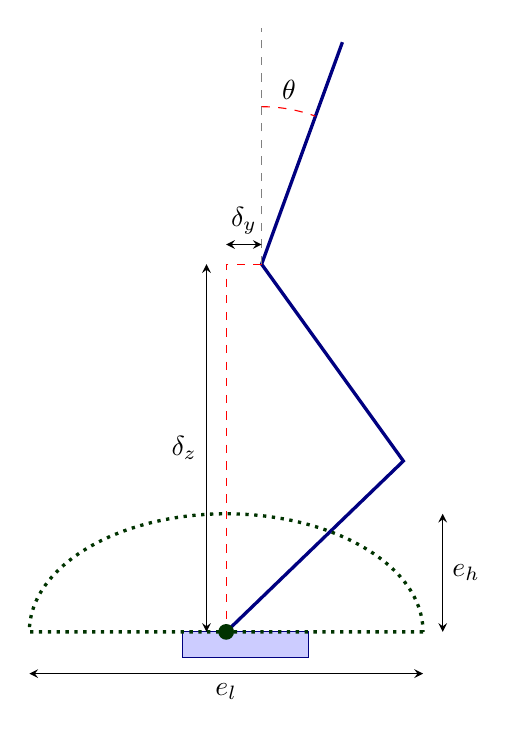
\begin{tikzpicture}[>=stealth]
    \filldraw[fill=white!80!blue,draw=black!50!blue] (-.8,0) rectangle (.8,.33);
    
    \draw[black!50!blue,very thick] (-.25,.33) -- (2,2.5) -- (0.2,5) -- ++(70:3);
    \draw[dashed, red] (0.2,5) -- (-.25,5) -- (-.25,.33);

    \draw[dotted,very thick,black!80!green] (2.25,0.33) -- (-2.75,0.33) arc(180:0:2.5 and 1.5);

    \fill[black!80!green] (-.25,.33) circle(0.1);

    \draw[help lines,dashed] (0.2,5) -- (0.2,8);
    \draw[dashed, red] (0.2,7) arc(90:80:2)  node[above,black]{$\theta$} arc(80:70:2);
    \draw[<->] (-2.75,-0.2) -- node[below]{$e_l$} (2.25,-0.2);
    \draw[<->] (2.5,0.33) -- node[right]{$e_h$} (2.5,1.83);
    \draw[<->] (-.5,0.33) -- node[left]{$\delta_z$} (-.5,5);
    \draw[<->] (-.25,5.25) -- node[above]{$\delta_y$}(0.2,5.25);
  \end{tikzpicture}
  \caption{Visualization of the IK gait and its parameters.
    joint. The green dotted line shows the path that the feet follows
    (not that actually the path is defined in coordinates of the ankle
    joint). This path is characterized by the {\tt ellipseheight}
    ($e_h$) and {\tt ellipselength} ($e_l$) parameters. The position
    of the pathe relative to the agent's hip is determined by the {\tt
      offsety} and {\tt offsetz} parameters ($\delta_y$ and $\delta_z$
    respectively). Finally, the {\tt leanangle} ($\theta$) parameter
    determines how far the torso should additionally lean
    forward. \label{fig:gait}}
\end{figure}

This figure show some of the parameters that determine the actual
resulting path. These parameters can be configured in the XML
configuration file; the full list and the XML element names to be used
can be found in Tab.~\ref{tab:ikparams}. Again, for a working example,
look at the {\tt DribbleAgent} example agent code, and it's XML
configuration file.

\begin{table}
  \begin{tabular}{cll}
    Param & XML & Description \\
    \hline
    $T$ & {\tt period} & Time to complete 2 steps: one with each leg (seconds). \\
    $\tau$ & {\tt startuptime} & Time to reach full speed/step sizes from standstill (seconds). \\
    $e_l$ & {\tt ellipselength} & Maximum ellipse length/step size (meters). \\
    $e_h$ & {\tt ellipseheight} & Maximum ellipse/step height (meters). \\
    $e_w$ & {\tt sidewidth} & Maximum sideways step size (meters). \\
%    $d_x$ & {\tt offsetx} & Offset of ellipse center from hip along x-axis, in meters. (\emph{currently ignored}). \\
    $d_y$ & {\tt offsety} & Offset of ellipse center from hip along y-axis (meters). \\
    $d_z$ & {\tt offsetz} & Offset of ellipse center from hip along z-axis (meters). \\
    $\alpha_{max}$ & {\tt maxturnangle} & Maximum angle for {\tt LEG1} joint, used to turn (degrees). \\
    $\theta$ & {\tt leanangle} & Angle of torso relative to vertical (degrees).
  \end{tabular}
  \caption{List of {\tt IKGaitGenerator} configurable parameters \label{tab:ikparams}}
\end{table}

%%% Local Variables: 
%%% mode: latex
%%% TeX-master: "libbatsmanual"
%%% End: 
